\section{Evaluation Approach}
\label{sec:eval_approach}
    As acknowledged in Chapter~\ref{chapter:conclusions}, \textit{Glosy} has not yet been evaluated in a controlled study with human learners. This is the main disadvantage of the present work: none of the results in this chapter can speak to actual vocabulary gain, retention, or engagement, since no learner has yet used the system under observation. In the absence of that evidence, this chapter instead evaluates the system's own algorithmic components directly, against real seeded content, to establish whether each behaves as its design in Chapter~\ref{methodology} intends and where it does not --- a necessary but not sufficient substitute for pedagogical evidence, and one that Chapter~\ref{chapter:conclusions} returns to among its directions for future work. Each section below targets one component in isolation, using the real, unmodified implementation from Chapter~\ref{chapter:discussion} rather than a re-derived model of it.

\section{Component-Level Algorithmic Evaluation}
\label{sec:component_eval}

    \subsection{Word of Wonders: Grid-Generation Benchmark}
    \label{subsec:wow_eval}

    The crossword placement algorithm of Section~\ref{subsec:wow_impl} (Algorithms~\ref{alg:wow_placement} and~\ref{alg:wow_priority}) is bounded by three constants: an $8\times8$ board, a practice-word length of at most 8 letters, a shared letter-budget of 8 distinct-letter slots (\texttt{MAX\_LETTERS\_LENGTH}), and a cap of 12 placed words (\texttt{MAX\_WORDS}). Because the algorithm's behaviour depends on how large and how diverse a candidate word pool it is asked to search, and a learner's tracked vocabulary grows from a handful of words at first use to potentially thousands after months of use, the two questions this evaluation asks are: does the generator remain robust as tracked vocabulary grows, and how do the two quantities that matter to a learner --- how rich the resulting puzzle is, and how long they wait for it --- scale with that growth.

    \subsubsection{Method}
    \label{subsubsec:wow_eval_method}
    A benchmark harness (\texttt{scripts/evaluation/wow\_generator/} in the project repository) imports \texttt{LevelGenerator.js} unmodified and drives it with word pools sampled directly from the seeded per-language dictionaries of Section~\ref{sec:data_modelling} (13,373 English, 13,722 Greek, and 14,315 Farsi entries). For each of the three supported languages and seven simulated tracked-vocabulary sizes (10, 100, 500, 1{,}000, 3{,}000, 6{,}000, and 10{,}000 words --- the last comfortably exceeding what any real learner's tracked vocabulary reaches in practice, to characterise the algorithm's behaviour at the extreme rather than only the typical case), 200 repetitions drew an independent random subset of that size from the full dictionary, selected one of its words uniformly at random as the FSRS-due practice word (mirroring \texttt{GameLoader.js}'s own unfiltered selection --- Section~\ref{subsec:game_review_design}), and called the generator exactly as the application does. This produced 4{,}200 trials in total, recording the words placed, the wall-clock generation time, and whether an exception was raised.

    \subsubsection{Robustness}
    Across all 4{,}200 trials, at every vocabulary size in every language, the generator raised no exception and always returned a non-empty board with its practice word placed. This holds even at the smallest tested vocabulary (10 words), where the candidate pool for intersecting words is thin, and at the largest (10{,}000 words), where the priority sort and intersection search run over a considerably larger candidate pool per call than any real session is likely to present it with.

    \subsubsection{Words Placed}
    \label{subsubsec:wow_eval_words_placed}
    \begin{figure}[htbp]
        \centering
        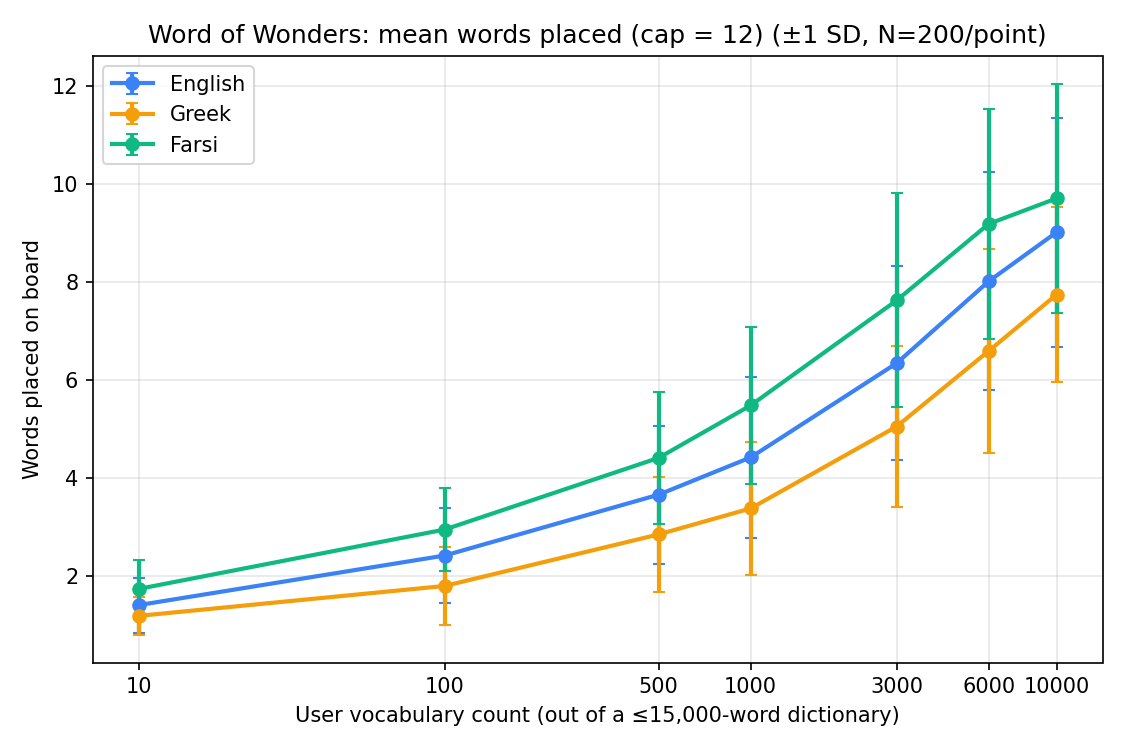
\includegraphics[width=0.8\textwidth]{figures/wow_words_placed.png}
        \caption{Mean words placed on the board (cap = 12) as a function of simulated tracked-vocabulary size, per language. Error bars show $\pm 1$ standard deviation over 200 repetitions per point.}
        \label{fig:wow_words_placed}
    \end{figure}
    Figure~\ref{fig:wow_words_placed} shows words placed rising with vocabulary size in all three languages, from a mean of 1.2--1.8 words at a 10-word vocabulary to 7.7--9.7 words at 10,000 --- yet even at that extreme, the board never saturates the 12-word cap. This confirms the design argument of Section~\ref{subsec:wow_design}: the binding constraint on puzzle richness is the 8-slot letter budget of \texttt{wouldExceedLetterLimit}, not the word count or the cap itself, since a bigger, more diverse candidate pool exhausts the shared letters faster than it exhausts the word cap. A second, consistent pattern across every vocabulary size is a language ordering --- Farsi places the most words, English second, Greek fewest --- consistent with average word length: among the words the generator accepts (three to eight letters after normalisation), the mean length is 5.1 letters for Farsi, 6.0 for English, and 6.5 for Greek, so the language with the shortest words places the most, since a longer average word consumes more of the same 8-letter budget per placement.

    A direct consequence for onboarding is that a brand-new learner, whose tracked vocabulary is by construction small, is served a sparse board of only one or two words rather than a filled one --- compounding, rather than mitigating, the "steep onboarding barriers" limitation already acknowledged in Chapter~\ref{chapter:conclusions}.

    \subsubsection{Qualitative Example: On-Device Boards Across CEFR Levels}
    \label{subsubsec:wow_eval_screenshots}
    \begin{figure}[htbp]
        \centering
        \begin{subfigure}[b]{0.31\textwidth}
            \centering
            
\includegraphics[width=\linewidth]{figures/wow_screenshot_a1.jpg}
            \caption{A1}
            \label{fig:wow_shot_a1}
        \end{subfigure}\hfill
        \begin{subfigure}[b]{0.31\textwidth}
            \centering
            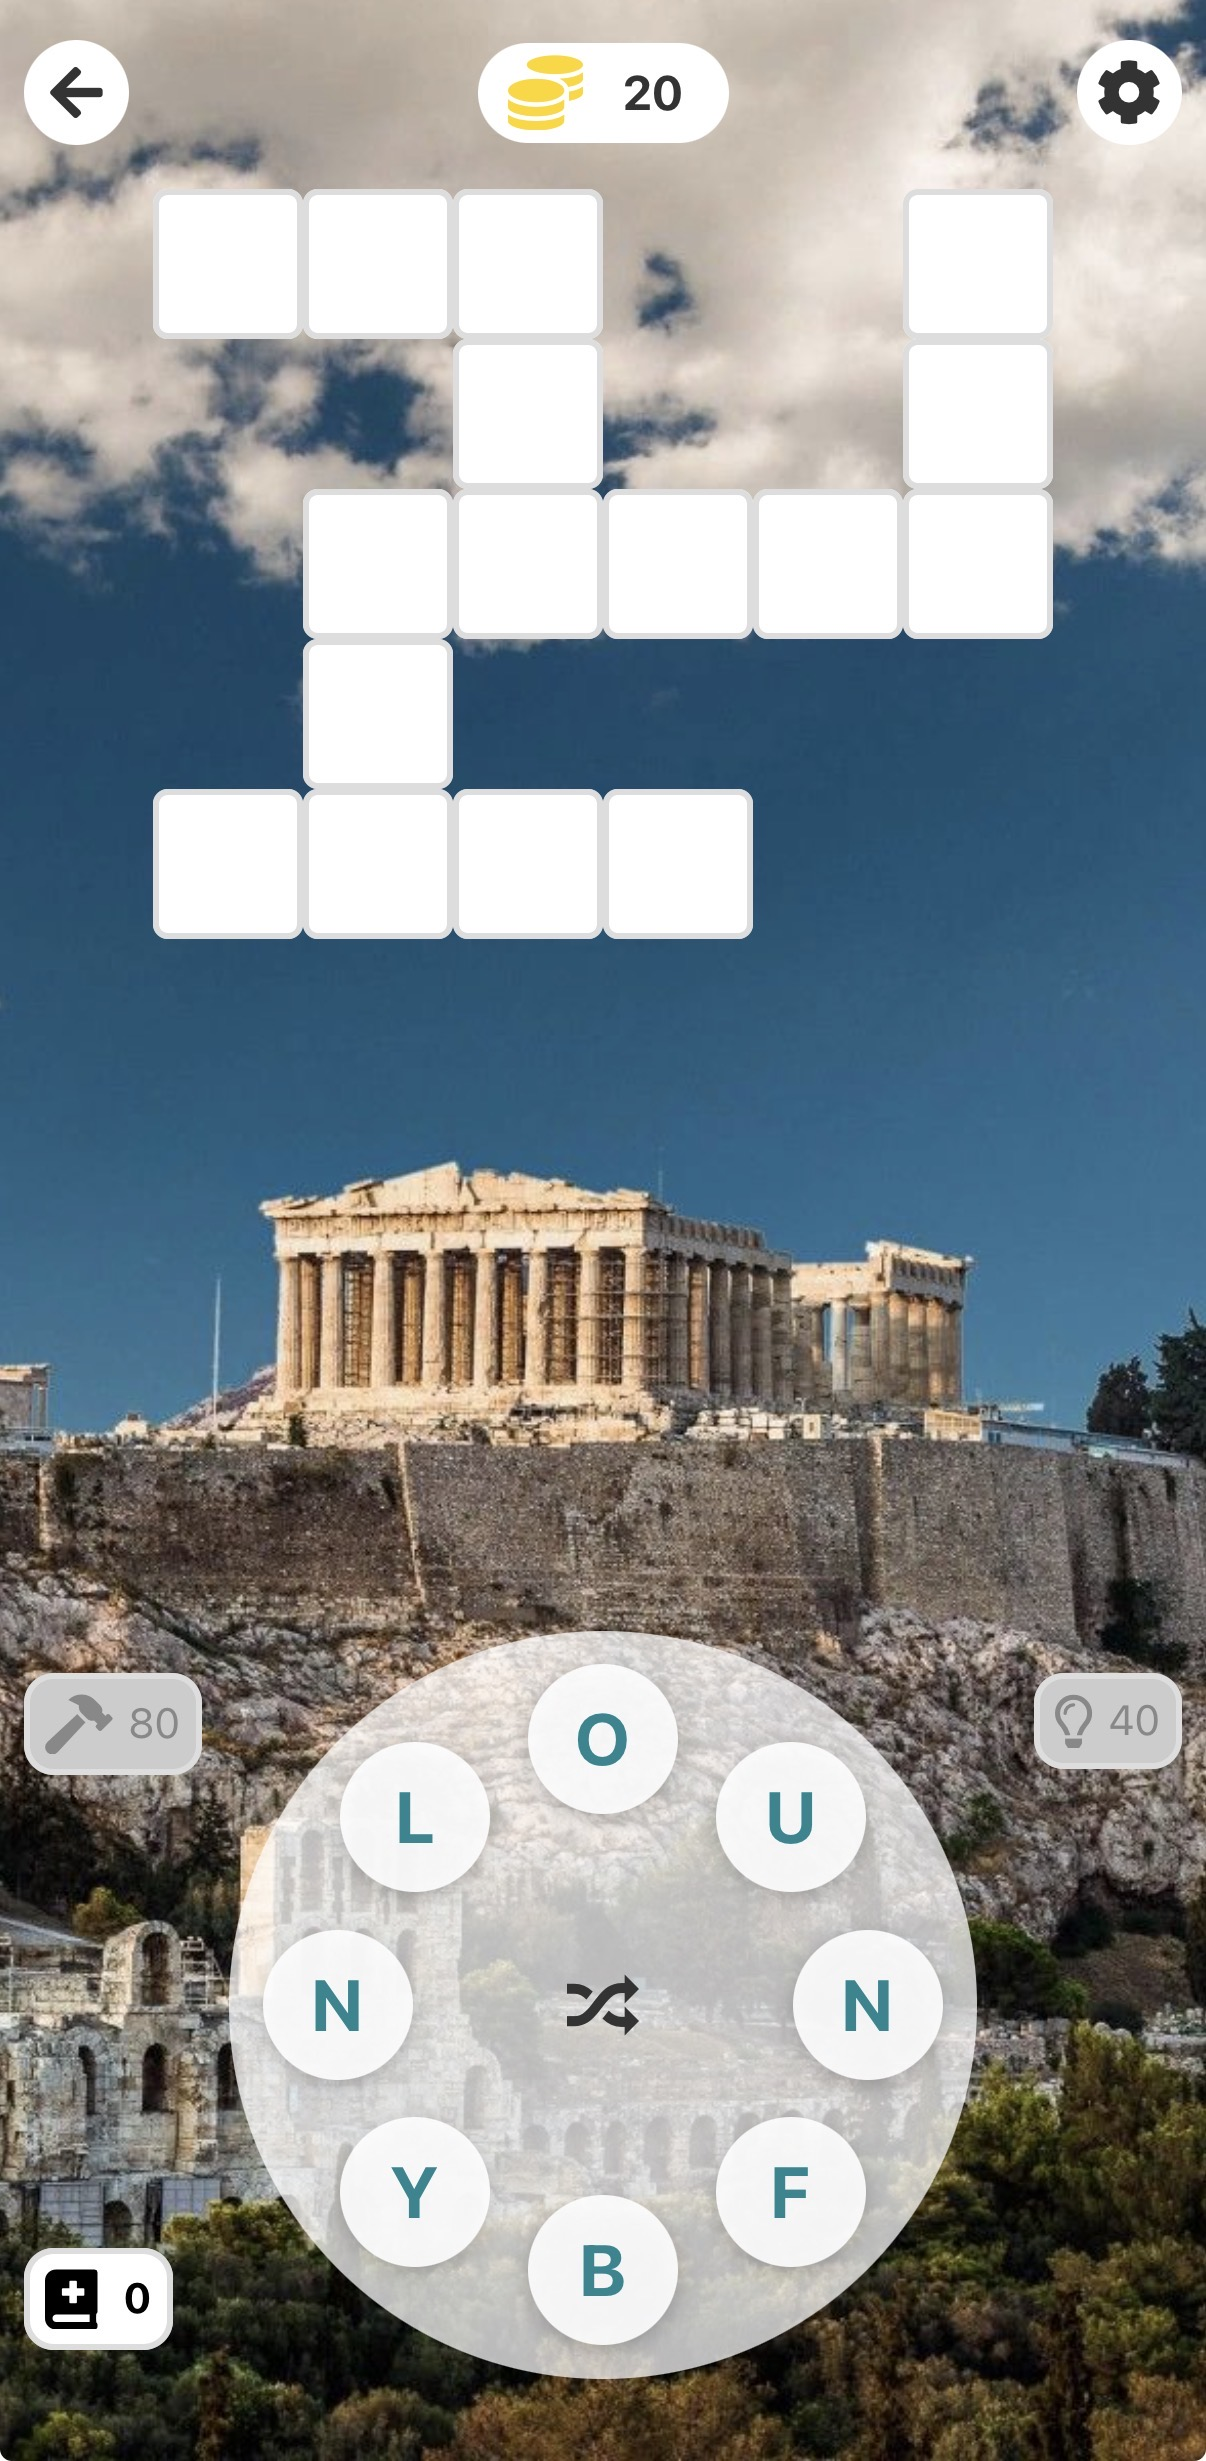
\includegraphics[width=\linewidth]{figures/wow_screenshot_a2.jpg}
            \caption{A2}
            \label{fig:wow_shot_a2}
        \end{subfigure}\hfill
        \begin{subfigure}[b]{0.31\textwidth}
            \centering
            
\includegraphics[width=\linewidth]{figures/wow_screenshot_b1.jpg}
            \caption{B1}
            \label{fig:wow_shot_b1}
        \end{subfigure}

        \vspace{1\baselineskip}

        \begin{subfigure}[b]{0.31\textwidth}
            \centering
            
\includegraphics[width=\linewidth]{figures/wow_screenshot_b2.jpg}
            \caption{B2}
            \label{fig:wow_shot_b2}
        \end{subfigure}\hfill
        \begin{subfigure}[b]{0.31\textwidth}
            \centering
            
\includegraphics[width=\linewidth]{figures/wow_screenshot_c1.jpg}
            \caption{C1}
            \label{fig:wow_shot_c1}
        \end{subfigure}\hfill
        \begin{subfigure}[b]{0.31\textwidth}
            \centering
            
\includegraphics[width=\linewidth]{figures/wow_screenshot_c2.jpg}
            \caption{C2}
            \label{fig:wow_shot_c2}
        \end{subfigure}
        \caption{Word of Wonders boards generated on a physical device for an English learner who declared each of the six CEFR levels at onboarding, all other conditions held fixed. Board density visibly grows from a bare two-word cross at A1 to a multi-armed board of several intersecting words by B2--C2.}
        \label{fig:wow_screenshots_cefr}
    \end{figure}
    Figure~\ref{fig:wow_screenshots_cefr} shows the same generator running on a physical device, for one learner who selected each of the six CEFR levels in turn. The pattern corroborates Figure~\ref{fig:wow_words_placed} directly, but through a different mechanism than the benchmark's own uniform random sampling: proficiency-based vocabulary auto-seeding (Section~\ref{subsec:registration_impl}) inserts every word at every level \emph{below} the learner's declared one into \texttt{user\_vocabulary} at registration, so declaring A1 --- already the lowest level --- seeds nothing and leaves \texttt{GameLoader.js}'s \texttt{trackedWords} pool empty of anything beyond whatever the learner has reviewed since, while declaring C2 seeds the entire A1--C1 dictionary at once. The visibly sparse A1/A2 boards and the visibly denser B2--C2 ones are therefore a real instance of the same word-count effect Section~\ref{subsubsec:wow_eval_words_placed} measured synthetically, produced by the application's actual onboarding path rather than by the benchmark harness.

    \subsubsection{Generation Time}
    \label{subsubsec:wow_eval_gen_time}
    \begin{figure}[htbp]
        \centering
        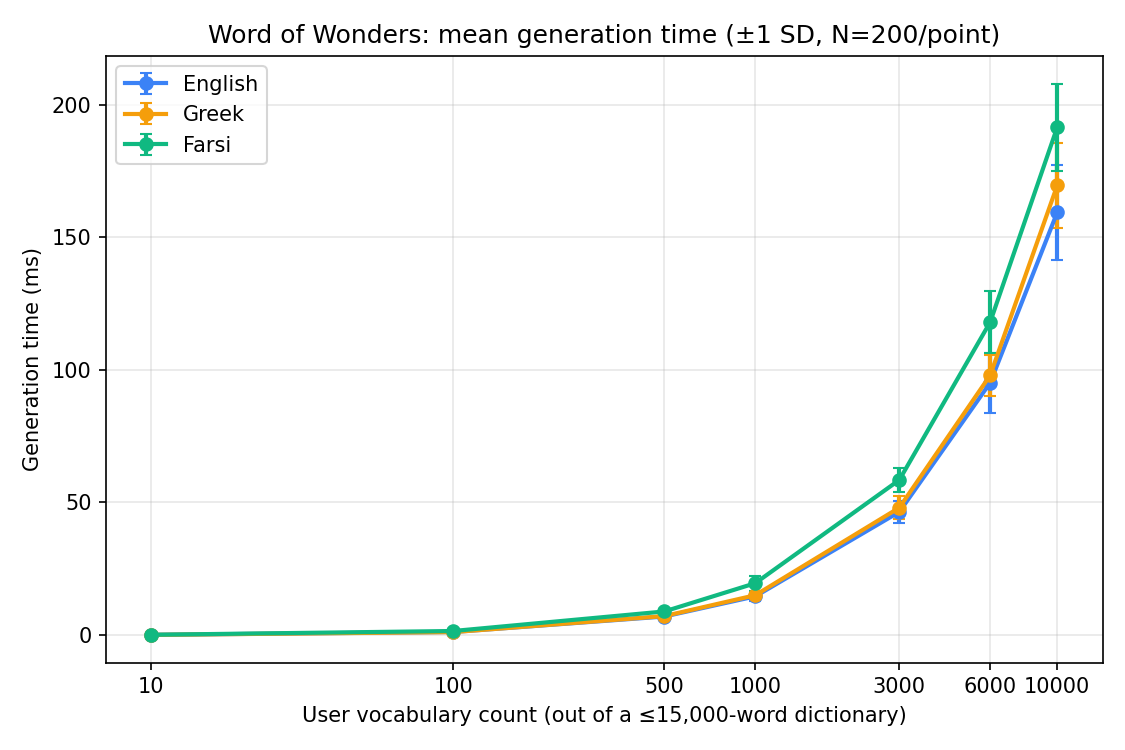
\includegraphics[width=0.8\textwidth]{figures/wow_generation_time.png}
        \caption{Mean grid-generation wall-clock time (ms) as a function of simulated tracked-vocabulary size, per language, measured under Node.js/V8 on a development machine. Error bars show $\pm 1$ standard deviation over 200 repetitions per point.}
        \label{fig:wow_generation_time}
    \end{figure}
    Figure~\ref{fig:wow_generation_time} shows generation time growing from sub-millisecond at a 10-word vocabulary to 159--192~ms at 10,000 words, with the three languages tracking each other closely throughout. The curve is visibly superlinear beyond roughly 3,000 words, consistent with \texttt{tryPlaceWord}'s per-candidate intersection search scaling with both the number of words already placed and the priority sort (Algorithm~\ref{alg:wow_priority}) running over the entire candidate pool on every call.

    These figures were measured under Node.js/V8 on a laptop, not under Hermes on an actual mobile device, and are reported here as evidence of the algorithm's \emph{scaling behaviour} --- no combinatorial blow-up and no failure at any tested scale --- rather than as a prediction of on-device latency: JIT and garbage-collection behaviour differ enough between V8 and Hermes, and between individual phones, that an absolute millisecond figure measured on one device would not transfer to another. \texttt{GameLoader.js} currently calls the generator synchronously on the JS thread (Section~\ref{subsec:wow_impl}), wrapped only in a zero-delay \texttt{setTimeout} to yield a render frame for the loading spinner, not to move the computation off-thread; the superlinear growth observed here means that a learner whose tracked vocabulary eventually reaches the thousands of words could, on slower hardware, experience a visibly longer wait than the benchmark's low-vocabulary numbers suggest. A direct mitigation, left as a concrete direction rather than spec here, is to move grid generation server-side --- the reels service's existing infrastructure (Section~\ref{sec:reels_service_impl}) already performs comparable per-request computation --- and push a precomputed board to the client opportunistically the next time it is online, trading a network round trip for a guaranteed, device-independent generation cost rather than an open question per phone.

    \subsection{Recommendation Engine: The Cold-Start Problem}
    \label{subsec:recommender_cold_start}
    Cold start --- a recommender system having little or nothing to personalise on for a given user --- is a well-known limitation of collaborative and content-based recommendation alike, not a defect specific to \textit{Glosy} \cite{adomavicius2005toward}. Section~\ref{subsec:cascade_hybrid} already gave this as the reason the engine has no collaborative-filtering stage at all: a cross-learner interaction matrix dense enough to be useful does not yet exist for a newly-launched application. What this section evaluates is how the same problem manifests one level down, inside Stage~3 itself, and what \textit{Glosy} currently does and does not do about it.

    Stage~3's profile vector (Section~\ref{subsec:stage3_design}) is built entirely from \texttt{reel\_interactions} --- the weighted sum of the TF-IDF vectors of reels a learner has liked, saved, shared, or commented on. Since every one of \textit{Glosy}'s current users is, by definition, a user who has not yet accumulated that history, \texttt{profile\_vector} is \texttt{None} for all of them today, and Section~\ref{subsec:cascade_design}'s graceful degradation takes over: the cascade's sort key collapses to (has-due-word, constant~0), i.e. Stage~2 plus a random tiebreak, with Stage~3 contributing nothing. This is not a rare edge case the design merely tolerates --- it is, at present, the actual ranking behaviour for the entire user base, for as long as no one has interacted with enough reels to build a profile from.

    \textit{Glosy} already has a partial, in-progress answer to this in its onboarding flow, one screen ahead of where the cascade could use it. The last onboarding page (\texttt{PersonalizationSlide.tsx}, Figure~\ref{fig:onboarding_personalization}) asks the learner to multi-select from a fixed set of eight topic chips --- Movies, Sports, Anime, Make up, Cartoons, Video games, News, Politics --- and to declare an age (16 upward, matching the declared Play Store audience), both required before onboarding can proceed. Both are persisted at registration: \texttt{preferences} as a comma-joined string and \texttt{age} as an integer, both columns on \texttt{users} (Section~\ref{sec:data_modelling}). Neither, however, is read anywhere in \texttt{reel\_service.py} --- not in Stage~3's profile construction, not anywhere else in \texttt{get\_personalized\_reels} or \texttt{get\_random\_reels}. The data is collected and stored; the recommendation engine simply does not look at it yet. This is a genuine gap rather than a documentation lag: the schema and the onboarding UI are already ahead of the recommendation code that would consume them.

    \begin{figure}[!htbp]
        \centering
        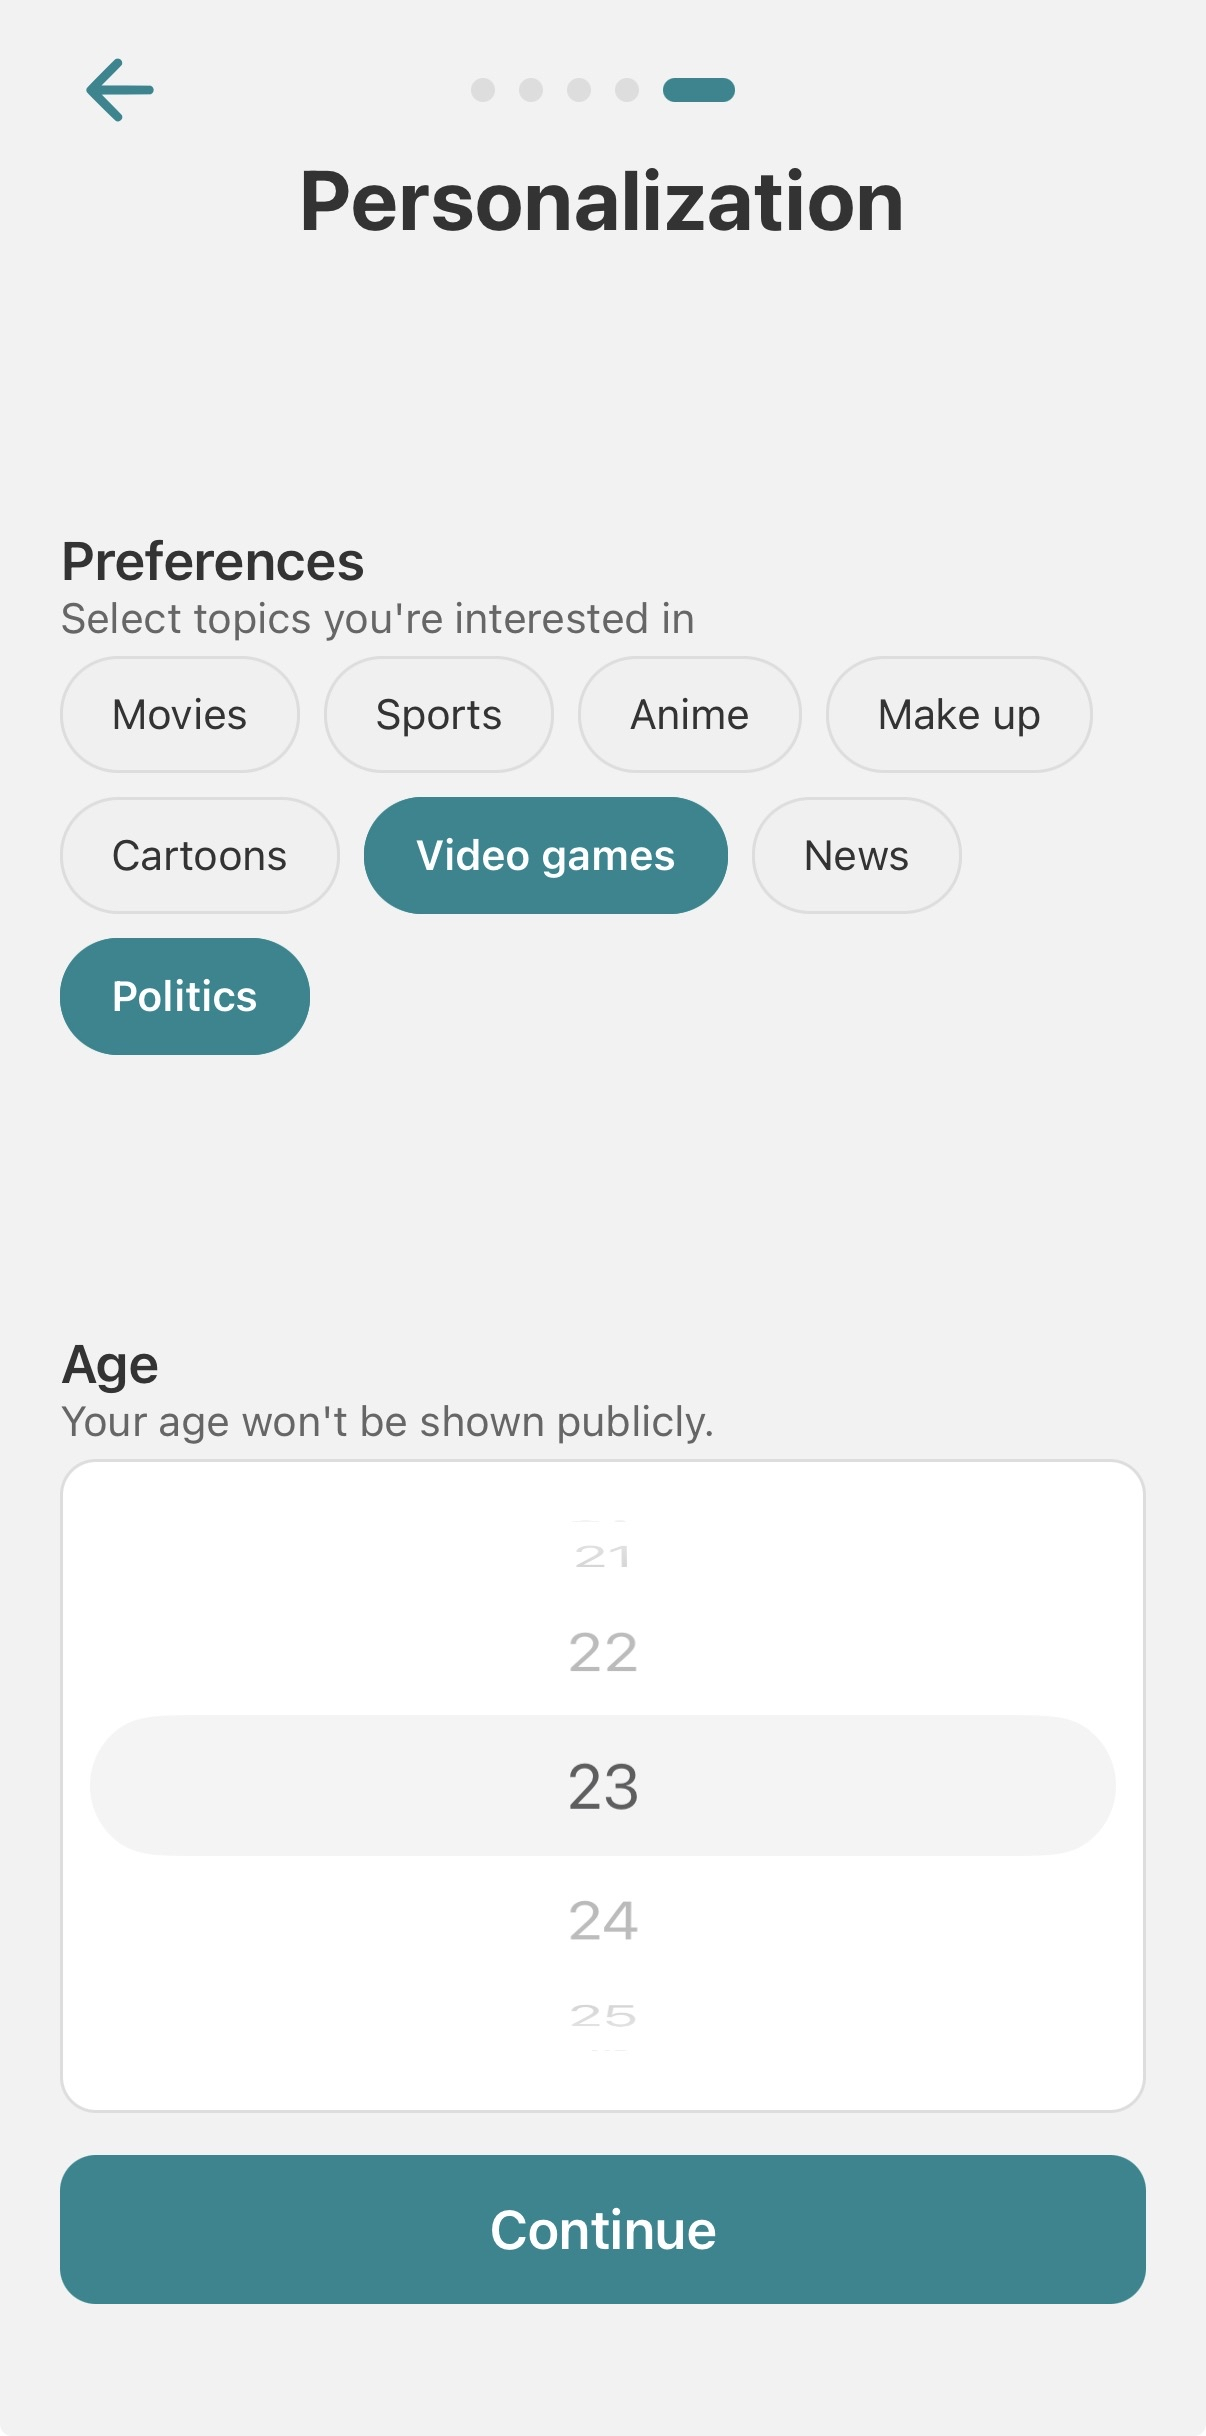
\includegraphics[width=0.28\textwidth]{figures/onboarding_personalization.jpeg}
        \caption{The Personalization screen (\texttt{PersonalizationSlide.tsx}), the last onboarding page}
        \label{fig:onboarding_personalization}
    \end{figure}

    Two concrete directions follow directly from this gap, both already anticipated by the existing structure rather than requiring a new data model: first, using the declared topic preferences as a cold-start substitute for Stage~3's profile vector --- a sensible prior for a learner who has stated an interest in, say, Sports, before they have liked a single reel, closing the gap identified in the paragraph above --- currently limited by the fixed, hand-picked eight-topic taxonomy the onboarding chips offer, with automated topic generation (deriving topics from reel content rather than a static hardcoded list) as the natural next step once a large enough content library makes that worth building; and second, age-conditioned recommendation, using the already-collected \texttt{age} column as a further ranking or filtering signal once a concrete policy for it is designed. Chapter~\ref{chapter:conclusions} is updated to carry both forward as named future-work items.

    \subsection{Recommendation Engine: Stage 1 Comprehensibility Filter}
    \label{subsec:stage1_eval}
    Stage~1's outcome (Section~\ref{subsec:stage1_design}) depends less on the filter itself than on the catalogue it is applied to: how many reels exist for the learner's language, how densely each reel's subtitles are tokenised (a reel with no tokenised word can never pass), and how many reels were recently recommended to the learner, since these are excluded for a 24-hour cooldown window. The results below are therefore illustrative rather than a property of the engine alone. The catalogue currently holds only 56 Farsi reels, inserted only to show how the filter behaves rather than curated as a learning library; 50 of the 56 have at least one tokenised word, and the other six can never pass yet.

    \begin{figure}[!htbp]
        \centering
        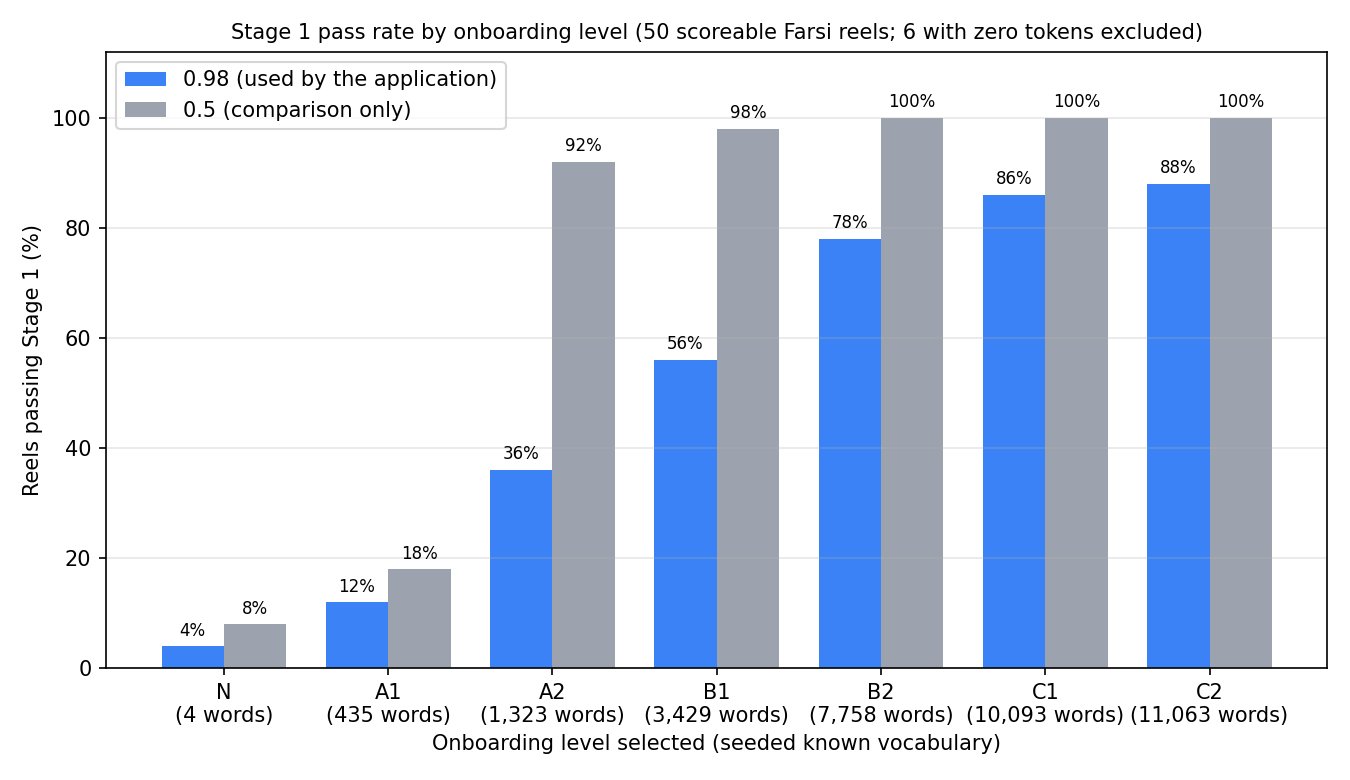
\includegraphics[width=0.80\textwidth]{figures/stage1_pass_rate.png}
        \caption{Share of the 50 tokenised Farsi reels passing Stage~1, per onboarding level, at the threshold the application uses (0.98) and, for comparison only, a looser one (0.5). Each level's known vocabulary is what registration seeds for it (Section~\ref{subsec:registration_impl}); level N receives only four starter words.}
        \label{fig:stage1_pass_rate}
    \end{figure}

    Figure~\ref{fig:stage1_pass_rate} shows that at the 0.98 threshold the application uses, beginners are barely served (level N: 4\%; A1: 12\%), the pass rate rises through A2 (36\%) and B1 (56\%), and it reaches only 88\% even at C2. For comparison, Stage~1 was also evaluated at a looser threshold of 0.5, which saturates from A2 upwards (92\%) but still passes only 8\% and 18\% of reels for levels N and A1. A looser filter therefore does not close the beginner gap: that needs easier content, not a lower threshold, and the application keeps the 0.98 threshold.

    \subsection{Recommendation Engine: Stage 2 Due-Word Prioritisation}
    \label{subsec:stage2_eval}
    Stage~2 (Section~\ref{subsec:stage2_design}) can only prioritise reels if the learner has words due for review. A learner who declares level N for Farsi has no lower level to seed vocabulary from, so onboarding instead adds four everyday starter words --- \textit{sal\={a}m} (hello), \textit{\={a}b} (water), \textit{b\={a}b\={a}} (dad) and \textit{ch\={a}y} (tea) --- as brand-new FSRS cards, all due immediately. The catalogue of 56 Farsi reels was assembled so that reels containing these words exist: 11 of the 56 contain at least one of them (\textit{sal\={a}m} in 5, each of the other three in 2).

    The scenario tested is a new user who has not registered and opens the reels feed. The frontend forwards the four due words with the request, and for a guest the server applies Stage~2 alone, since the comprehensibility filter and the content-based ranking both need an account. Running the reels service's own ranking and review-word assignment code on the real catalogue, over 2{,}000 repetitions, every reel on the first page of ten contains a due word, against 1.96 of ten for a page requested without due words, and all four words receive a review prompt on every page, each attached to a different reel. The mechanism therefore behaves as designed, but only because the catalogue was built around these four words: it holds just 11 such reels, so a second page can carry at most one more. As with Stage~1, what limits the feature is the size of the catalogue, not the ranking logic.

    \subsection{Recommendation Engine: Stage 3 Content-Based Ranking}
    \label{subsec:stage3_eval}
    Stage~3 (Section~\ref{subsec:stage3_design}) is not tested here. It is built entirely on scikit-learn's TF-IDF weighting and cosine similarity, an established library implementing a long-standing retrieval technique, so re-testing those components would evaluate the library rather than \textit{Glosy}. What remains specific to the system, its dependence on an interaction history that no user has yet accumulated, is discussed in Section~\ref{subsec:recommender_cold_start}.
